%情報処理学会全国大会原稿テンプレート ver. 1.2

\documentclass[uplatex,twocolumn]{jsarticle}
\usepackage[top=30mm,bottom=25mm,left=20mm,right=20mm]{geometry}
\usepackage[T1]{fontenc}
\usepackage{txfonts}
\usepackage[expert,deluxe]{otf}
\usepackage[dvipdfmx,hiresbb]{graphicx}
\usepackage[dvipdfm]{hyperref}
\usepackage{pxjahyper}
\usepackage{multicol}
\setlength{\columnsep}{7mm}

\title{\vspace{-10mm}\Large{大学入試センター試験数学Ⅰ・Aを用いた数式処理システムの性能評価}\footnotemark[0]}
\author{\large{森谷 慧士\footnotemark[2]\qquad 矢吹 太朗}\\千葉工業大学 社会システム科学部 プロジェクトマネジメント学科\footnotemark[3]}
\date{}
\pagestyle{empty}
\begin{document}
\twocolumn[\maketitle]

%脚注の追加をするために以下を追加
\begingroup
\def\thefootnote{\fnsymbol{footnote}}
\footnotetext[0]{Performance evaluation of symbolic computation system in solving National Center Test for University Admissions math problems.}%要修正(最後はピリオド)
\footnotetext[2]{Satoshi Moriya (s1242116nc@s.chibakoudai.jp)}%要修正
\footnotetext[3]{Department of Project Management, Faculty of Social Systems Science, Chiba Institute of Technology.}
\endgroup



\section{序論}

東京大学の入試問題を全自動で解くプロジェクト(東ロボプロジェクト)が進められている\cite{arai2014}.その処理システムは,大学入試センター試験(以下では,センター試験と記載する)の模擬試験(5教科8科目)で950満点中511点(偏差値は57.8)を獲得,数学と世界史の偏差値は特に高く,数学Ⅰ・A は偏差値64,数学Ⅱ・Bは偏差値65.8,世界史は偏差値66.5であったという\cite{tourobo}.

人工知能がこのように発達すると,その影響は数学教育にも及ぶだろう.今日の数学教育は,すべてを紙と鉛筆で行うことを前提に行われているが,その一部はコンピュータで置き換えることができるはずである.人間が行うこととコンピュータが行うことをうまく識別する能力の育成が求められるようになるだろう.

\section{目的}

本研究では,大学入試センター試験数学I・Aを題材にして,数学教育にコンピュータを導入することの可能性を調査する.その結果として,高校程度の数学能力を問う問題をコンピュータを活用して解く際に必要となる数学の知識とコンピュータの知識を明らかにすることを目指す.





\section{手法}

本研究では,センター試験の数学I・Aの問題をコンピュータを用いて解き,問題を解くために必要な数学の知識とコンピュータの知識を確認する.

\subsection{センター試験}
2009年から2015年までの7年分のセンター試験の数学I・Aの問題を解く.

\subsection{コンピュータシステム}
解答にはコンピュータシステムは数式処理システムMathematicaを用いる.コンピュータを数学に応用する方法は,低水準言語から高水準言語まで,さまざまなレベルが考えられるが,本研究では,人間が書く答案と抽象度が最も近いと思われる数式処理システムを検討し,数式処理システムの中で最も普及しているものの一つであるMathematicaを採用する.Wolfram言語の実行環境をMathematicaと呼ぶこともあるが,本稿では言語自体もMathematicaと呼ぶ.
Mathematicaには,Windows版とMac版,Linux版,Raspberry Pi版,クラウドサービス版があるが,本研究では,無料で利用できるクラウドサービス版,Wolfram Programming Lab\footnote{\url{https://lab.open.wolframcloud.com/objects/wpl/GetStarted.nb}}を用いる.

\subsection{解答方法}
数式処理システムを用いて数学の問題を解く例として,「$x$についての方程式$f(x)=x^2-ax+5=0$が重解を持つような$a$の値を求めよ」という問題を,2通りの方法で解く.
第1の方法は,方程式が重解を持つことと判別式$a^2-20$が$0$であることが同値だと考え,$a$についての方程式$a^2-20=0$を解くというものである.方程式を解くためには,Mathematicaの\verb|Solve[|方程式\verb|, |変数\verb|]|という記法を用いる.\cite{wolfram2014}.

\begin{verbatim}
Solve[a^2 - 20 == 0, a]
\end{verbatim}
\vspace{-5mm}\[\left\{\left\{a\to -2 \sqrt{5}\right\},\left\{a\to 2 \sqrt{5}\right\}\right\}\]
この結果は,$a$が$-2\sqrt{5}$または$2\sqrt{5}$であることを表している.

第2の方法は,2次方程式が重解を持つということをMathematicaが処理可能な形式に変換し,その記述を評価するというものである.2次方程式が重解を持つというのは,「ある解$x_1$が存在し,すべての解$x_2$は$x_1$と等しい」と言い換えられる.この命題を論理式で書くと$\exists x_1\;f(x_1)=0\land\left(\forall x_2\;f(x_2)=0\to x_2=x_1\right)$となる.\verb|Exists|や\verb|ForAll|を使ってこの命題を記述し,そこから限定子を除去すると$a$の値が求まる.限定子の除去には\verb|Reduce|を用いる.

\begin{verbatim}
Reduce[
 Exists[x1, f[x1] == 0,
  ForAll[x2, f[x2] == 0, x2 == x1]],
 a]
\end{verbatim}
\vspace{-5mm}\[a=-2 \sqrt{5}\lor a=2 \sqrt{5}\]
この結果も,$a$が$-2\sqrt{5}$または$2\sqrt{5}$であることを表している.
センター試験の問題は,紙と鉛筆で解けるように作られているため,そこにコンピュータを持ち込んでももちろん解ける.本研究では,問題をなるべく素直に解釈して解くことにする.上述の例では,判別式を思いつかなければならない第1の解法よりも,問題の表現を機械的に翻訳すればよい第2の解法を採用する.


\subsection{集計}
問題を解いたら,その際に用いたMathematicaの組み込みシンボルの種類を数える.たとえば,上述の第2の解法では,\verb|Reduce|と\verb|Exists|,\verb|ForAll|という3種の組み込みシンボルを用いている(厳密に言えば,\verb|x2 == x1|は正式には\verb|Equal[x2, x1]|と記述されるため,\verb|Equal|も数えるべきではあるが,ここでは「\verb|==|」のような自明なものは数えないことにする).
初めのうちは,問題の数が増えるにつれて,利用する組み込みシンボルの種類も増えるが,センター試験の数学I・Aの問題を解くのに使える組み込みシンボルが出尽くせば,シンボルの種類の増加は止まるはずである.



\section{結果}
\begin{figure}[tb]
\centering
%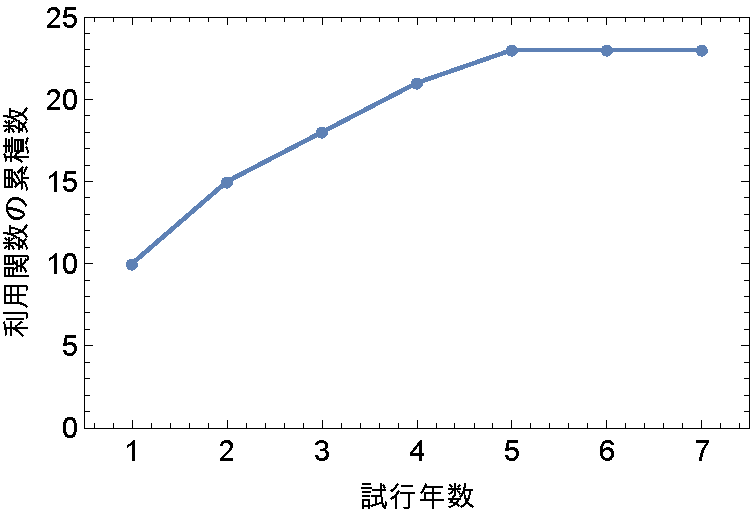
\includegraphics[width=\columnwidth]{code.pdf}
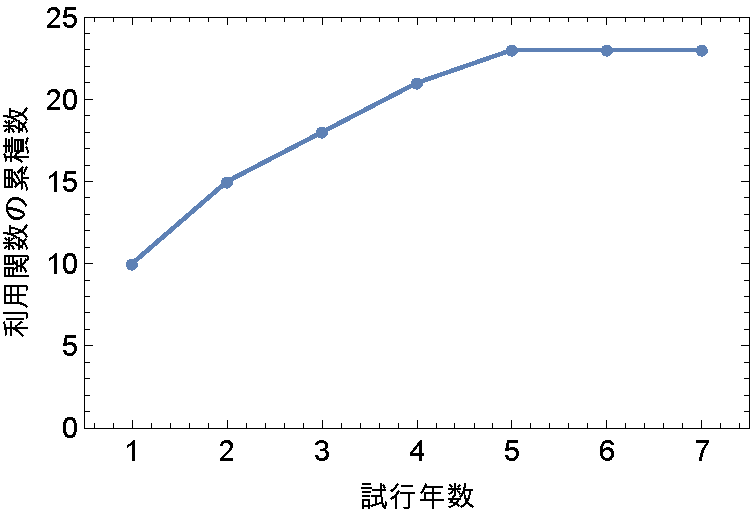
\includegraphics[scale=0.5]{code.pdf}
\caption{試行年数に対する使用関数の累積数}\label{累積グラフ}
\end{figure}

2009年から2015年までのセンター試験の数学Ⅰ・Aの問題を解き,利用したMathematicaの組み込みシンボルの累積数を記録した結果が図\ref{累積グラフ}である.
利用した組み込みシンボルは全部で23個となり,使用頻度順に,\verb|Solve|(方程式を解く),\verb|Reruce|(同値な式に置き換える),\verb|Simplify|(簡約),\verb|SolveAlways|(恒等式となる条件を求める),\verb|Maxmize|(最大化),\verb|TrigExpand|(三角関数を展開する),\verb|TrigFactor|(三角関数をまとめる),\verb|TrigReduce|(三角関数を書き換える),\verb|FactorInteger|(因数を取り出す),\verb|Divisors|(約数を求める),\verb|Length|(リストの長さを求める),\verb|Sqrt|(平方根),\verb|!|(階乗),\verb|Clear|(シンボル割り当ての解除),\verb|Integate|(積分),\verb|Factor|(因数分解),\verb|Cos|(余弦),\verb|Sin|(正弦),\verb|SetDelayed|(関数定義),\verb|Expand|(式の展開),\verb|HornerForm|(ホーナー形式への変換),\verb|Degree|(角度の変換)であった.

\section{考察}
組み込みシンボルの累積数の増加が図{累積グラフ}のように6年で止まったため,センター試験の数学I・Aの問題を解くのに必要なMathematicaの機能は,「結果」に記載した23種類で十分であることがわかる.Mathematicaのような数式処理システムには膨大な機能が備えられているが,数学I・Aのために必要なのはこのように比較的少数の機能があり,教育の現場に導入するのも容易だと思われる.

\section{結論}
本研究では,数式処理システムMathematicaを用いてセンター試験の数学Ⅰ・Aの問題を解いた.その際に利用したMathematicaの組み込みシンボルを集計することによって,センター試験の数学Ⅰ・Aを解くのに必要な数式処理システムについての知識を明らかにすることができた.本研究のような事例を増やすことによって,コンピュータのサポートのもとで数学の問題を解くのに必要な数学の知識を明らかにすることが今後の課題であろう.




\bibliographystyle{junsrt}
\bibliography{biblio}%「biblio.bib」というファイルが必要.

\end{document}